\chapter{PLANTEAMIENTO DEL PROBLEMA}
\section{Descripción de la Realidad Problemática}

En América Latina, la situación es igualmente preocupante. Un estudio realizado por la Comisión Económica para América Latina y el Caribe (CEPAL) reveló que el 60\% de los habitantes rurales no tienen acceso a servicios de salud adecuados \citep*{OECD_World_Bank_2020}. La falta de acceso a servicios de salud tiene consecuencias graves para la población pediátrica. La UNICEF informa que las tasas de mortalidad infantil en áreas rurales son significativamente más altas que en áreas urbanas. En países en desarrollo, los niños que viven en zonas rurales tienen el doble de probabilidades de morir antes de los cinco años en comparación con sus contrapartes urbanas \cite{Unicef}.

La situación de atención médica en las áreas rurales de Perú es una realidad compleja y desafiante. Imagine comunidades enclavadas en paisajes montañosos y remotos, donde acceder a servicios médicos básicos es una odisea. La falta de infraestructura adecuada y la escasez de profesionales de la salud crean una brecha significativa en el acceso a la atención médica, dejando a muchas personas sin la ayuda que necesitan cuando más la necesitan. Según el Instituto Nacional de Estadística e Informática (INEI), en 2022, solo el 20\% pertenece a la población rural, en comparación con el 80\% de la población urbana. Esto significa que millones de peruanos en áreas rurales son más vulnerables a enfermedades y muertes evitables.

\begin{figure}[h]
	\begin{center}
		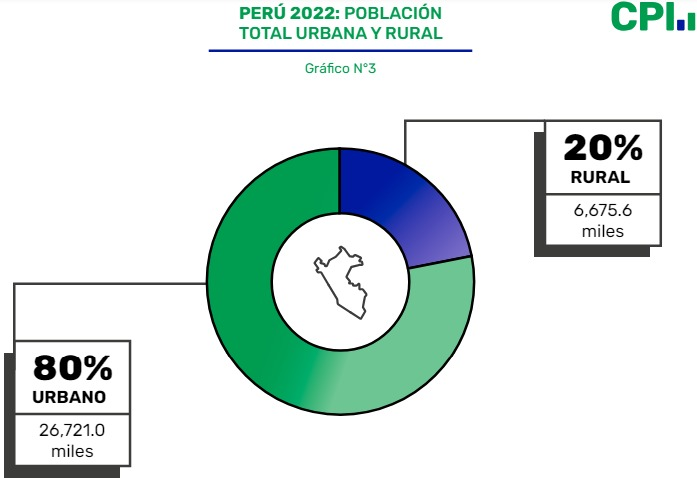
\includegraphics[width=0.6\textwidth]{1/figures/INEITOTAL.jpeg}
		\caption{Total de poblacion rural y urbana. Fuente: \cite{gl_inei}}
		\label{1:fig}
	\end{center}
\end{figure}

Ademas, los datos oficiales respaldan estas realidades duras. Según el Ministerio de Salud de Perú, en el 2021, más del 70\% de la población rural carecía de acceso regular a servicios médicos adecuados. Esto no es solo una estadística fría, sino una narrativa de vidas afectadas, enfermedades no tratadas y vidas que podrían haberse salvado con una atención médica oportuna.

\begin{figure}[h]
	\begin{center}
		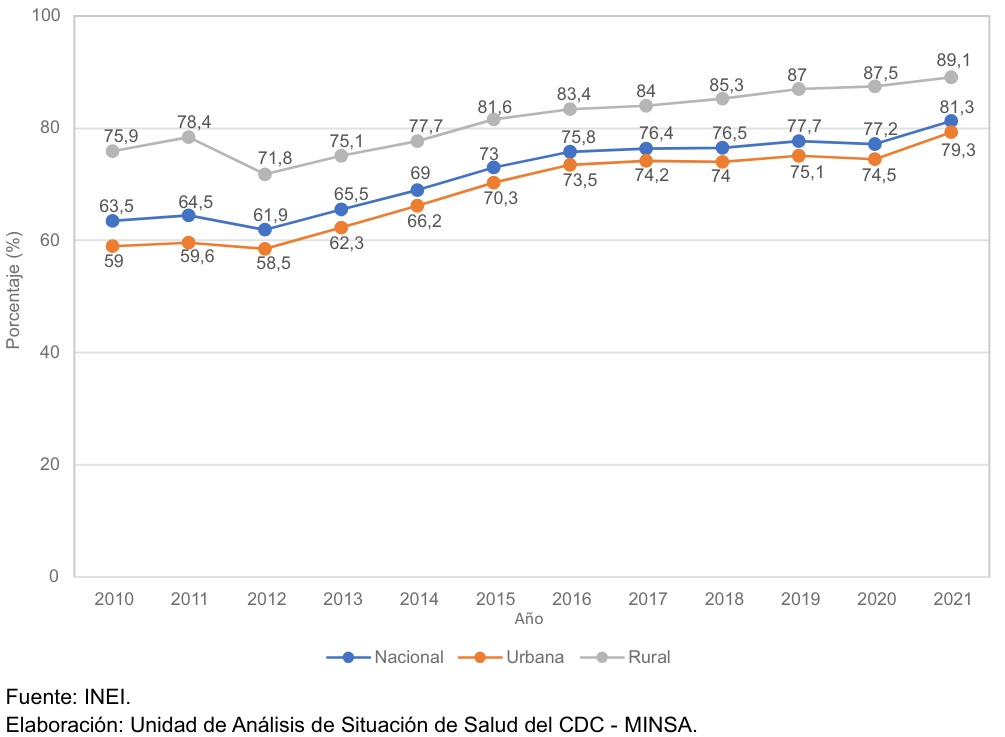
\includegraphics[width=0.6\textwidth]{1/figures/MINSA.jpeg}
		\caption{Porcentaje de acceso a atencion medica. Fuente: \cite{gl_inei}}
		\label{2:fig}
	\end{center}
\end{figure}
%\begin{figure}[h]
%	\begin{center}
	%		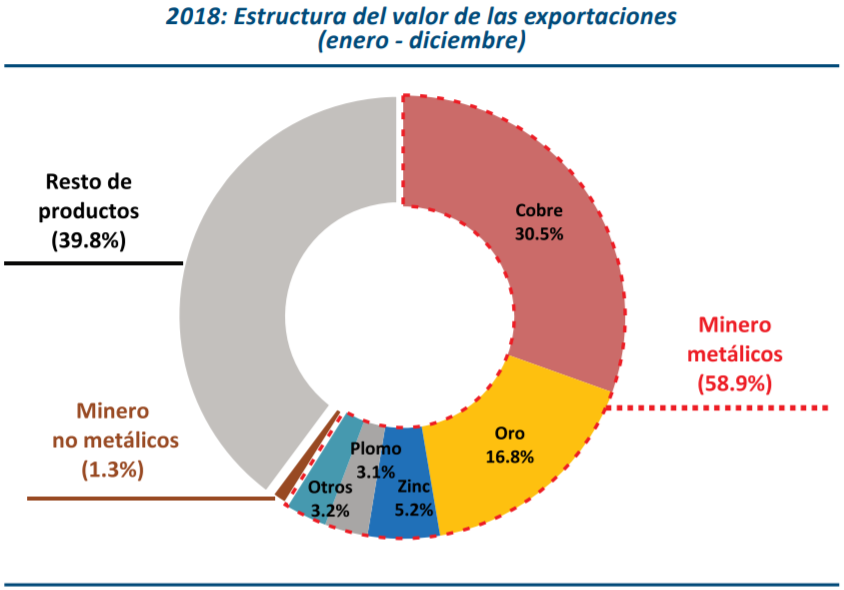
\includegraphics[width=0.8\textwidth]{1/figures/estructura_exportaciones_peru.png}
	%		\caption{Estructura del valor de las exportaciones peruanas en el año 2018. Fuente: \cite{cu_ministerioPeru_statsminas}}
	%		\label{1:fig2}
	%	\end{center}
%\end{figure}

Durante el período comprendido entre 2022 y 2024, la pandemia de COVID-19 solo ha intensificado estos desafíos. Los recursos y la atención se desplazaron hacia la respuesta a la pandemia, dejando otras necesidades de salud pública en segundo plano. Las comunidades rurales se encontraron aún más marginadas, enfrentando una atención médica aún más limitada y fragmentada.

Sin embargo, entre estas sombras de dificultades, hay un rayo de esperanza en la forma de la tecnología. El aumento del acceso a teléfonos móviles en áreas rurales ofrece una oportunidad única para brindar servicios médicos básicos a través de plataformas digitales, incluso en las zonas más remotas del país. Es aquí donde entra en juego la idea de un chatbot médico.

Imagínese un sistema donde las personas en las comunidades rurales pueden acceder a información médica básica, hacer consultas sobre síntomas y recibir orientación sobre cómo buscar atención médica, todo desde la comodidad de sus teléfonos móviles. Esto no solo podría salvar vidas, sino también aliviar la carga sobre los pocos centros de salud disponibles en estas áreas.

Pero, por supuesto, hay obstáculos por superar. La adaptación cultural, la capacitación de los usuarios y la garantía de la precisión de la información son solo algunos de los desafíos que enfrenta esta iniciativa. Además, la conectividad limitada en algunas áreas rurales plantea desafíos adicionales para garantizar un acceso efectivo a la aplicación.

La implementación de Chatbots Médicos en áreas rurales del Perú tiene el potencial de mejorar significativamente el acceso a la atención médica para millones de personas. Estos sistemas pueden proporcionar información y asesoramiento médico de manera remota, sin necesidad de que un médico esté presente físicamente. Además, los Chatbots Médicos pueden ayudar a los pacientes a programar citas, recordarles que tomen sus medicamentos y monitorear su progreso. 

%\begin{figure}[h]
%	\begin{center}
%		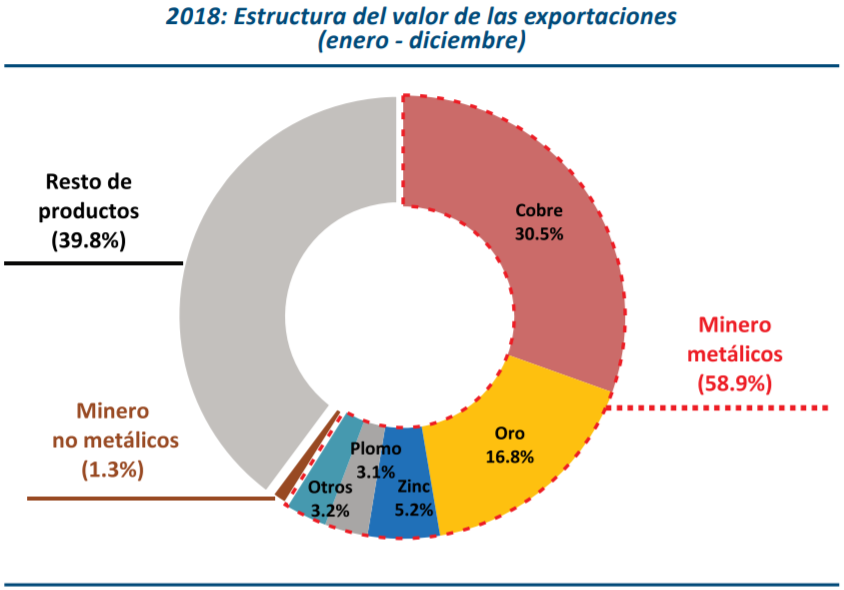
\includegraphics[width=0.8\textwidth]{1/figures/estructura_exportaciones_peru.png}
%		\caption{Estructura del valor de las exportaciones peruanas en el año 2018. Fuente: \cite{cu_ministerioPeru_statsminas}}
%		\label{1:fig2}
%	\end{center}
%\end{figure}

%\begin{figure}[h]
%	\begin{center}
%		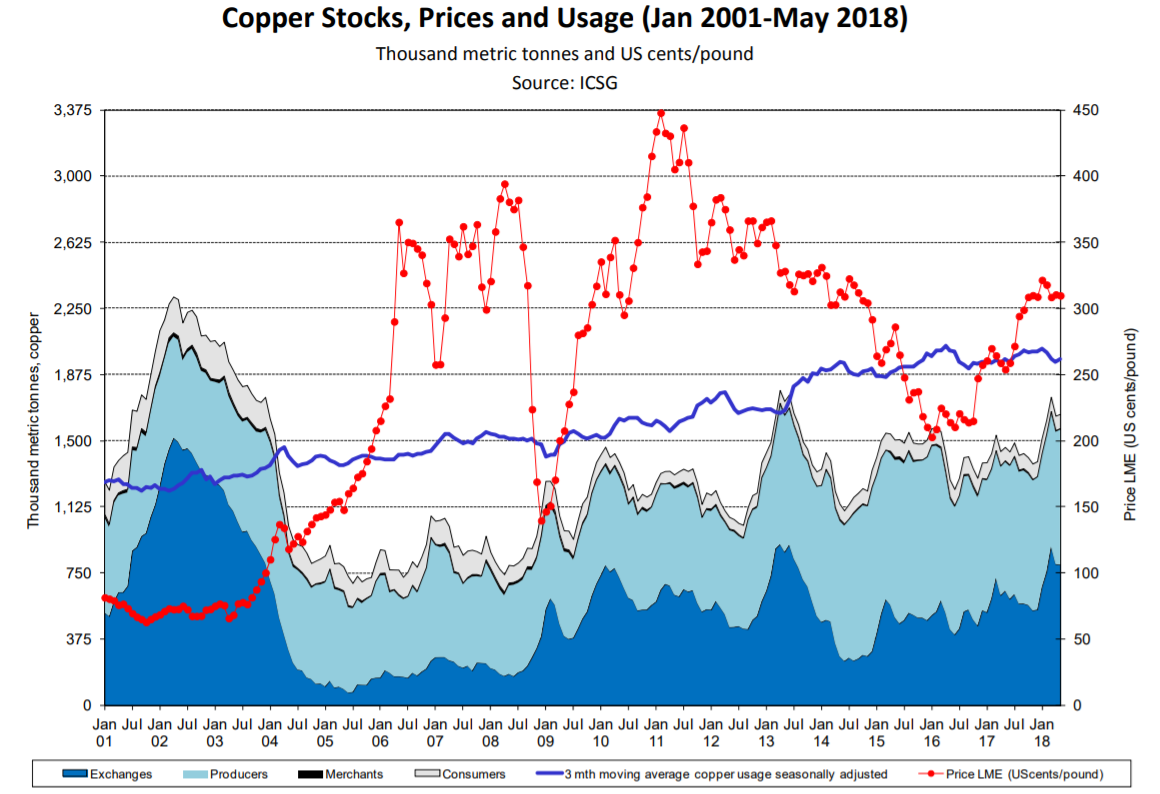
\includegraphics[width=0.8\textwidth]{1/figures/copper_stocks_prices_usage.png}
%		\caption{Precio, stocks y uso del cobre (cantidad en miles de toneladas y precio en centavos por libra). Fuente: \cite{cu_internationalcopper2018}}	
%		\label{1:fig3}
%	\end{center}
%\end{figure}

\section{Formulación del Problema}

%Para lefecto \parencite{ot_marti2018manual}. 


%Una vez elaborado el diagrama (véase Anexo 1), 

\subsection{Problema General}
\newcommand{\ProblemaGeneral}{
¿De qué manera la implementación de un chatbot médico puede mejorar el acceso a servicios de salud en las zonas rurales de Perú?
}
\ProblemaGeneral
\subsection{Problemas Espec\'{i}ficos}
\newcommand{\Pbone}{
¿Que datos disponibles se necesitaran para la implementacion de chatbot?
}
\newcommand{\Pbtwo}{
¿Que arquitectura podrían ser utilizadas para desarrollar un chatbot médico?
}
\newcommand{\Pbthree}{
¿Qué métodos de entrenamiento y validación se pueden utilizar para un chatbot?
}
\newcommand{\Pbfour}{
¿Qué métricas se pueden utilizar para evaluar la efectividad del chatbot médico?
}


\begin{itemize}
	\item \Pbone
	\item \Pbtwo
	\item \Pbthree
	\item \Pbfour

\end{itemize}

\section{Objetivos de la Investigación}

%Para la formulación de los objetivos de la presente investigación se elaboró un «árbol de objetivos» (véase Anexo 2) 
\subsection{Objetivo General}
\newcommand{\ObjetivoGeneral}{
Implementar un chatbot médico efectivo y sostenible para brindar servicios de salud de calidad a las poblaciones rurales en Perú
}
\ObjetivoGeneral
\subsection{Objetivos Espec\'{i}ficos}
\newcommand{\Objone}{
Identificar los datos disponibles y necesarios para la implementación del chatbot médico en áreas rurales de Perú.
}
\newcommand{\Objtwo}{
Explorar las diferentes arquitecturas disponibles para el desarrollo del chatbot médico.
}
\newcommand{\Objthree}{
Investigar métodos de entrenamiento y validación adecuados para un chatbot médico.
}
\newcommand{\Objfour}{
Definir métricas de evaluación para medir la efectividad y el impacto del chatbot médico en la prestación de servicios de la salud.
}

\begin{itemize}
	\item {\Objone}
	\item {\Objtwo}
	\item {\Objthree}
	\item {\Objfour}
\end{itemize}

\section{Justificación de la Investigación}

\subsection{Teórica}
La implementación de un chatbot médico en áreas rurales de Perú se fundamenta en varias teorías clave. La teoría de la difusión de innovaciones de \cite{rogers2003} es fundamental para entender cómo las nuevas tecnologías se adoptan dentro de una sociedad. Rogers argumenta que la adopción de innovaciones depende de la ventaja relativa, compatibilidad, complejidad, capacidad de prueba y observabilidad. Para un chatbot médico, la ventaja relativa se manifiesta en la capacidad para proporcionar atención médica inmediata y accesible. La compatibilidad se refiere a cómo esta tecnología se integra en la vida cotidiana y entorno cultural, mientras que la complejidad debe ser mínima para garantizar la facilidad de uso. La capacidad de prueba permite a usuarios experimentar con el chatbot, y la observabilidad se relaciona con los beneficios visibles que otros pueden percibir al usar la tecnología.

Además, la teoría del cuidado centrado en el paciente, promovida por \cite{Epstein100}, subraya la importancia de una atención personalizada y accesible. La atención médica debe adaptarse a las necesidades individuales de los pacientes, considerando sus valores y preferencias. En áreas rurales, un chatbot puede proporcionar un nivel de personalización y atención que de otra manera sería inalcanzable, mejorando significativamente la calidad de la atención y la satisfacción del paciente.

La teoría del acceso equitativo a la salud descrita por \cite{Braveman254}, menciona que todas las personas, independientemente de su ubicación geográfica o condición socioeconómica, deben tener acceso a servicios de salud de calidad. En Perú, las disparidades en el acceso a la atención médica entre las áreas urbanas y rurales son marcadas. Un chatbot médico puede actuar como un nivelador, proporcionando información y asistencia médica, reduciendo así las inequidades en salud.

\subsection{Práctica}
Los chatbots pueden proporcionar información médica confiable y oportuna a los pacientes. En áreas rurales, donde el acceso a profesionales de la salud es limitado y las instalaciones médicas a menudo están lejos, un chatbot puede actuar como una primera línea de consulta médica. Esto puede ayudar a los pacientes a recibir orientación inmediata sobre sus síntomas, lo cual es crucial para la detección temprana y el manejo adecuado de enfermedades.

Además, la implementación de un chatbot médico puede mejorar la eficiencia del sistema de salud. Los chatbots pueden automatizar la respuesta a preguntas frecuentes y proporcionar diagnósticos preliminares, lo que puede reducir la carga de trabajo de los profesionales de la salud y permitirles centrarse en casos más complejos. Esto es especialmente relevante en situaciones de emergencia y en el manejo de enfermedades crónicas, donde el monitoreo constante y el acceso rápido a la información son vitales.

Un estudio realizado por \cite{Pricewaterhouse} destacó que los chatbots pueden ayudar a reducir los costos en el sector de la salud al mejorar la eficiencia y la gestión de los recursos. En áreas rurales de Perú, donde los recursos son escasos y el acceso a la atención médica es limitado, esta tecnología puede ser un cambio transformador. Los pacientes pueden obtener la ayuda que necesitan de manera rápida y eficiente, lo que puede mejorar los resultados de salud y reducir las tasas de complicaciones y hospitalizaciones.

Además, la implementación de un chatbot médico puede empoderar a los pacientes rurales al proporcionarles acceso a información médica confiable. Esto puede aumentar su conocimiento sobre su propia salud y fomentar prácticas de autocuidado, lo cual es crucial en comunidades donde la educación en salud puede ser limitada. Al tener acceso a información precisa y recomendaciones médicas, los pacientes pueden tomar decisiones más informadas sobre su salud y bienestar.

\subsection{Metodológica}

Esta investigación se justifica por la oportunidad de desarrollar un modelo integral de implementación de chatbots médicos. El desarrollo del chatbot seguirá un enfoque de diseño centrado en el usuario \cite{Norman1986}, con iteraciones constantes y pruebas de usabilidad para asegurar una interfaz intuitiva. Una vez desarrollado, se realizará un estudio piloto que combinará análisis cuantitativos (como tiempos de respuesta y satisfacción del paciente) con análisis cualitativos de la experiencia del usuario.

Además, se podrán validar técnicas y herramientas innovadoras como el NLP, Machine Learning y el diseño de interacciones conversacionales naturales. Como señalan \cite{pr_Tudor_Car2020-jg}, $"$El uso de NLP y ML es clave para desarrollar chatbots médicos precisos y efectivos".

Otro aspecto metodológico importante es la generación de datos empíricos y evidencia científica sobre la aceptación, uso y efectividad del chatbot médico en comunidades rurales. Por lo que, se va a requerir más estudios de campo para evaluar el potencial de los chatbots de salud. Los datos generados en esta investigación podrían sentar las bases para futuros estudios y mejoras en la tecnología.

Finalmente, el desarrollo de métricas y herramientas de evaluación será fundamental para medir el desempeño e impacto del chatbot médico. Como sugieren \cite{pr_Abd-Alrazaq2020-ct}, $"$Es necesario contar con métricas específicas para evaluar la efectividad de los chatbots de salud en cuanto a la calidad de la información, la satisfacción del usuario y los resultados clínicos". Estas métricas y herramientas podrían ser aplicadas en futuras investigaciones y proyectos similares.

\section{Delimitación del Estudio}

\subsection{Espacial}
La presente investigación se delimita espacialmente a las áreas rurales del Perú, las cuales presentan características geográficas, demográficas y socioeconómicas particulares que obstaculizan el acceso a servicios de salud. Según el Instituto Nacional de Estadística e Informática \cite{gl_inei}, $"$En el año 2022, el 20\% de la población peruana residía en el área rural", concentrándose principalmente en la sierra y la selva. Estos territorios rurales se caracterizan por su dispersión geográfica y baja densidad poblacional, como señalan \cite{pr_Diez-Canseco2015-uh} en su análisis del uso de tecnologías móviles en salud rural: "Los principales desafíos son la falta de recursos, la fragmentación geográfica y las barreras culturales" (p. 2).

Asimismo, la diversidad étnica y cultural es un factor relevante, con presencia de poblaciones indígenas y comunidades nativas quechua-hablantes y aimara-hablantes, cuyas características socioculturales deben ser consideradas para asegurar la accesibilidad del chatbot médico.

\subsection{Temporal}
Esta investigación se desarrollará en un período de aproximadamente 2 años, con fases de diseño, desarrollo, implementación piloto y evaluación inicial del chatbot médico en comunidades rurales seleccionadas estratégicamente. Sin embargo, es importante considerar el contexto actual y proyecciones futuras.

Actualmente, el Ministerio de Salud de Perú (MINSA, 2022) ha implementado diversos programas y políticas orientadas a mejorar el acceso a servicios de salud en zonas rurales, como la Estrategia Sanitaria Nacional de Salud de los Pueblos Indígenas. Además, se han realizado esfuerzos por incorporar tecnologías como la telemedicina y los dispositivos móviles.

A futuro, se espera que la implementación del chatbot médico pueda escalarse a otras regiones rurales del país, integrándose con estrategias y tecnologías emergentes en el sector salud, como los sistemas de información geográfica y la inteligencia artificial aplicada a la medicina.

\subsection{Conceptual}
Según \cite{pr_Laranjo2018-gb}, un chatbot médico es un programa de computadora basado en inteligencia artificial diseñado para simular una conversación inteligente con usuarios humanos a través de canales de texto o voz, con el objetivo de brindar información y consejos médicos. Este tipo de tecnología ha ganado relevancia en los últimos años, ya que puede ayudar a superar barreras de acceso a servicios de salud, especialmente en áreas remotas y rurales.

Tomando como referencia el marco conceptual propuesto por \cite{pr_Levesque2013-vb}, el acceso abarca dimensiones como la accesibilidad geográfica, la disponibilidad, la aceptabilidad y la capacidad de pago. En el contexto de las áreas rurales peruanas, donde existen grandes desafíos en términos de dispersión geográfica, escasez de profesionales de la salud y barreras culturales, es esencial abordar estas dimensiones para lograr un acceso equitativo y efectivo a los servicios de salud.

Asimismo, la investigación se centrará en analizar los factores que influyen en la adopción y aceptación tecnológica del chatbot médico por parte de las poblaciones rurales. Para ello, se utilizará el Modelo Unificado de Aceptación y Uso de Tecnología (UTAUT) desarrollado por \cite{pr_Venkatesh2003-po}, el cual integra factores como la expectativa de desempeño, la expectativa de esfuerzo, la influencia social y las condiciones facilitadoras. Comprender estos factores será clave para diseñar e implementar el chatbot de manera efectiva y promover su adopción por parte de los usuarios.

Finalmente, la investigación también considerará los determinantes sociales de la salud, los cuales influyen en el estado de salud y el acceso a servicios médicos en las comunidades rurales

\section{Hipótesis}

\subsection{Hipótesis General}
\newcommand{\HipotesisGeneral}{
La implementación de un chatbot médico mejorará significativamente el acceso a servicios médicos de calidad para las poblaciones rurales.
}
\HipotesisGeneral
\subsection{Hipótesis Específicas}
\newcommand{\Hone}{
La disponibilidad de datos y la integración de APIs adecuadas serán fundamentales para el desarrollo exitoso del chatbot médico.
}
\newcommand{\Htwo}{
La arquitectura permitirá la creación de un chatbot médico eficiente y preciso.
}
\newcommand{\Hthree}{
La aplicación de métodos de entrenamiento y validación apropiados garantizarán la funcionalidad y confiabilidad del chatbot médico
}
\newcommand{\Hfour}{
La evaluación de métricas específicas revelará el impacto positivo del chatbot médico en la prestación de servicios de salud en áreas rurales de Perú
}
\begin{itemize}
	\item \Hone
	\item \Htwo
	\item \Hthree
	\item \Hfour

\end{itemize}

\subsection{Matriz de Consistencia}
A continuación se presenta la matriz de consistencia elaborada para la presente investigación (véase Anexo \ref{1:table}).

